\chapter{Noun phrases}
\label{ChapterNP} 
\is{Noun Phrase}

Vamale noun phrases, like verb phrases, are head-initial. Thus, noun phrases are composed in the following way: \gl{art}=\gl{psm} \gl{art}=\gl{psr}, optionally with relative clauses following each noun. Clitics flag noun phrases that are not object arguments, or unmarked intransitive subjects. %Exceptions to the rule that the first element is the head are 
%The examples in (\ref{ex:alignment}) show that the subject marking on active verbs, which include \textit{ta} \qu{go up} and all transitive verbs such as \textit{xaleke} \qu{to see}, displays nominative/accusative alignment, as do the free pronouns. 
Noun phrases display nominative-accusative alignment. \is{Alignment!Noun phrases}
This is typical of canonic Oceanic languages \parencite[495]{ross_morphosyntactic_2004}. Free pronouns can be flagged, like nouns, for the roles of transitive subject and intransitive subject, both obligatorily with \textit{ka} \qu{\gl{sbj}}, while nouns can omit \textit{ka} in intransitive scenarios, see (\ref{ex:opt_ka}). Personal pronouns can be flagged as oblique, but they cannot be used as undergoer arguments, contrary to nouns and demonstrative pronouns, e.g. \textit{ena} and \textit{nienaen}. Flagging is discussed in \sectref{sec:Casmark}.
\is{Alignment}
\ea \label{ex:opt_ka}
(No \textit{ka} before \textit{hmape-thoatit} \qu{cloud})\\
\gll cama vi hapi a=moo a=sibu ta-me \textbf{ka} i=jati nya-xahut hai cama hu-pe ca=hmape-thoatit a= xada\\
 \gl{subr} say \gl{comp} 3\gl{sg}=stay 3\gl{sg}=swell go.up-\gl{dir.cp} \gl{sbj} \gl{def}.\gl{sg}=sea towards-down.there or if come.down-\gl{dir.cp} \gl{indf}.\gl{sg}=flesh-sky \gl{rel}= up.there\\
\glt \qu{If one said (=let's imagine) that the sea down there should swell and rise, or that some cloud up there should come down [and shatter us, we shall still do custom]...} {[CP2:7]}
\z

In unmarked scenarios, \gl{p} and \gl{s} are marked the same way, meaning that both undergoer and intransitive subject noun phrases follow the verb without flagging, as shown in (\ref{ex:flagNP1}, \ref{ex:flagNP2}). Transitive subject noun phrases (\gl{a}), by contrast, are obligatorily marked by \textit{ka} \qu{\gl{sbj}} (\ref{ex:flagNP3}). This yields a tripartite alignment for nominal flagging, see \Cref{fig:alignment3}. The particle \textit{ka}, however, may also occur optionally with \gl{S\textsubscript{A}} and \gl{S\textsubscript{P}} (hence the gloss \qu{\gl{sbj}}). Note that this optional focusing use is not described for other languages in the area, suggesting it might be a relatively recent development.


\ea\label{ex:flagNP1}
\gll {\ob}a=han {\ob}i=xhaohmu{\cb\cb}  \\
 3\gl{sg}=walk \gl{def}.\gl{sg}=elder\\
\glt \qu{[The elder] walks.}
\z 

\ea\label{ex:flagNP2}
\gll {\ob}a\textsubscript{i}=xaleke {\ob}i=xhaohmu{\cb}\textsubscript{{\upshape ii}}{\cb}\\
 3\gl{sg}=see \gl{def}.\gl{sg}=elder\\
\glt  \qu{[S/he]\textsubscript{i} [sees [the elder]\textsubscript{ii}].}
\z 

\ea\label{ex:flagNP3}
\gll a=xaleke i=xhaohmu ka=ya\\
 3\gl{sg}=see \gl{def}.\gl{sg}=old \gl{sbj}=3\gl{sg}\\
\glt \qu{He sees the elder.}
\z

\begin{figure}
% % % 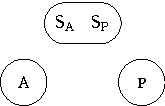
\includegraphics[width=0.3\linewidth]{figures/noun_alignment}
	\begin{tikzpicture}
		\topleftnode[sa]{\gl{S\textsubscript{A}}}
		\toprightnode[sp]{\gl{S\textsubscript{P}}}
		\leftnode[a]{\gl{a}}
		\rightnode[p]{\gl{p}}
		\draw (a) circle (11.2pt);
		\draw (p) circle (11.2pt);
		\draw \convexpath{11.2pt}{sa,sp};
	\end{tikzpicture}
	\caption{Alignment of noun phrase flagging}
	\label{fig:alignment3}
\end{figure}

Noun phrases can be formed by nouns, which were discussed in the previous \chapref{ChapterNouns}, but also by personal and demonstrative pronouns, which are described in \sectref{sec:Pronouns}. Apart from possessive constructions, discussed in the previous chapter (\sectref{sec:Poss}), nouns are chiefly modified by verbs and relative clauses. \sectref{sec:ModNoun} explores the morphemes within a noun phrase that modify the head, including adjective-like derivations (\sectref{sec:adj}). Noun phrases can be coordinated and form a new constituent. Vamale distinguishes at least three: the comitative \textit{ma}, the additive coordinator \textit{ka} \qu{also, on top of that}, and \textit{hai} \goodtilde \textit{a} \qu{or}. They are all described in \sectref{sec:CordNP}.

 \section{Case marking}
\label{sec:Casmark}
\is{Case}

Case in this grammar refers to the marking of syntactic roles by morphemes. Vamale, like most Oceanic languages \parencites[37]{lynch_oceanic_2002}[496]{ross_morphosyntactic_2004}, does not mark syntactic roles on nouns with affixes. There are, however, prepositions that ``flag" the subject (\textit{ka}) and optional, oblique arguments (\textit{(nya)ko}). The choice of the morphemes is influenced by semantic and pragmatic factors: transitive subject noun phrases must be preposed by \textit{ka} (further discussed in \sectref{ssec:ka}), whereas intransitive subject nouns may take \textit{ka} in focused contexts. Oblique markers distinguish beneficiary and goal arguments from more generically patientive ones (see \sectref{sec:oblique}), and are sensitive to the animacy of the argument.

\subsection{Agentive marker \textit{ka} }
\is{Case!Agentive}
\label{ssec:ka}

This \textit{ka} is a subject marker (\ref{ex:sbj marker}).\footnote{The Pije cognate to the agentive marker is \textit{lu}.} Its allomorph \textit{a} is conditioned by a final consonant on the preceding word. It is obligatory before nouns and pronouns that agree with the verb in an \textbf{A} function, probably because unmarked transitive subjects can occur at the very end of long VOS sentences, and directly after an object noun phrase: 

\ea V (VV\ldots) O \textit{ka} A. \z

\noindent A clitic \textit{ka} is optional for S\textsubscript{A/P}, probably in an extension of the first scenario. In principle, Vamale participant flagging is a tripartite flagging system, since it disambiguates A, which must take \textit{ka}, from S, which may take \textit{ka}, from O, which may not take \textit{ka} (see \Cref{fig:alignment3}). %In nominalizations, this changes: while \textit{ka} is obligatory for A, and optional for both S and O (provided A is not explicit) (\ref{ex:nmlz ka}). 

\ea
\label{ex:sbj marker}
%	% \langinfo{}{}{} 
\gll 	{\ob}e=xaleke i={\ob}jili i=bwaakala{\cb\cb} ka yo	\\
	{[}1\gl{sg}=see \gl{def}.\gl{sg}=[build\_with\_wood \gl{def}.\gl{sg}=canoe]] \gl{sbj} 1\gl{sg}	\\
\glt  \qu{I see the building of the canoe.}		
\z

%\ea\label{ex:nmlz ka}
%
%%\langinfo{}{}{} The Oué family
%\gll	i hun-xale-a ka yo	
%	\gl{def}.\gl{sg}=\gl{nmlz}-see-3\gl{obj} \gl{sbj} 1\gl{sg}
%\glt	\qu{My way of seeing him (lit. the way of see him by me)}

%\a
%
%%\langinfo{}{}{} The following can be grammatical, if the unmarked A \textit{yo} is pronounced as a different clause or as an adjunct (pause, lower intonation of \textit{yo}). \textit{yo} must be flagged with \textit{ka} if it is to be part of the same clause as the verb. 
%\gll 	*{[}e=xaleke i [jili i bwaakala]] yo	
%	1\gl{sg}=see \gl{def}.\gl{sg}=build\_with\_wood \gl{def}.\gl{sg}=canoe \gl{sbj} 1\gl{sg}	
%\glt  (for: \qu{I see the building of the canoe})	
%

%\a
%
%\langinfo{}{}{} (\textit{e}- is a bound pronoun, \textit{yo} its free form)
%\gll e=xale-le ka yo	
% 1\gl{sg}-see-3\gl{pl} \gl{sbj} 1\gl{sg}	
%\glt \qu{I see them} (lit. \qu{i-see-them by I})	
%


Contrary to A arguments, which have to be marked with \textit{ka} unless fronted and thus not part of the clause anymore (e.g. \textit{yo, e=xale-a} \qu{me, I see them}, see \sectref{sec:fronting}), S arguments do not have to be marked with \textit{ka} (\ref{ex:optional_ka}).

\ea \label{ex:optional_ka}
\gll a=hup-wa (ka) i=jati\\
 3\gl{sg}=go.down-\gl{rep} (\gl{sbj}) \gl{def}.\gl{sg}=sea\\
\glt \qu{The tide goes down again.}
\z

\ea
\gll sinu (ka) mu=xho-ng\\
 suffer (\gl{sbj}) \gl{def}.\gl{du}=leg-1\gl{sg}.\gl{poss}\\
\glt \qu{My legs hurt.} (no index on \textit{sinu} because it is a stative verb)
\z


%``Mémoire en vue d'obtention de l'habilitation à diriger des recherches", Claire Moyse-Faurie, 2004
%
%can depend on TAM (Drehu), animacy (nemi), pronoun vs noun, transitivity.
%
%

%There is no copula (\textit{be}). Instead, Vamale juxtaposes a subject and a predicate (or a topic and a comment). The subject's only obligatory expression is the ``person marking index", a proclitic attached to the predicate. It can be omitted in imperative constructions and some other circumstances, such as same-subject coordinative clauses. The predicate includes TAM markers, which come between the preverbal subject marker and the predicate. 
%The fact that the subject NP can be left out and that the subject is a clitic (i.e phonologically and morphologically(?) part of the predicate) a problem for well-formedness conditions? xx

In nominalizations as well, \textit{ka} \qu{\gl{sbj}} obligatorily occurs to mark A (\ref{ex:nmlz-ka1}, \ref{a ka yo}). P may take a different \textit{ka} \qu{\gl{link}} when it is the only participant present in the construction (\ref{ex:nmlz-ka2}). If several participants co-occur, this option disappears, as the clause would otherwise become confusing. As this \textit{ka} only marks S and P, I gloss it subsequently as absolutive (see \sectref{kan}).


\ea\label{ex:nmlz-ka1}
\gll i=hun-saxhuti i=jaxhut nyanya-n-eong \textbf{ka} caacaa-n-eong	\\
 \gl{def}.\gl{sg}=\gl{nmlz}-narrate \gl{def}.\gl{sg}=story mother-\gl{poss}-1\gl{sg}.\gl{poss} \gl{sbj}  father-\gl{poss}-1\gl{sg}.\gl{poss}	\\
\glt \qu{my father's way of telling my mother's story}	
\z
%%todo check the ka glossing here

\ea\label{ex:nmlz-ka2}
\gll i=hun-vii (ka) i=jaxhut	\\
 \gl{def}.\gl{sg}=\gl{nmlz}-say \gl{link} \gl{def}.\gl{sg}=story	\\
\glt \qu{the way to say the story}	
\z

\ea\label{ex:nmlz-ka3}
\gll i=hun-moo (ka) i=mwa\\
 \gl{def}.\gl{sg}=\gl{nmlz}-be \gl{link} \gl{def}.\gl{sg}=house\\
\glt \qu{the nature of the house}
\z


\ea\label{a ka yo}
\gll	i=hun-xale-a ka yo	\\
	\gl{def}.\gl{sg}=\gl{nmlz}-see-3\gl{obj} \gl{sbj} 1\gl{sg}\\
\glt	\qu{my way of seeing him (lit. the way of seeing him by me)}
\z 


%\begin{comment}
%Stuff with -\textit{n} in \ref{ex:no n} has to with specificity. -n is generic, absence of -n means a specific (but not necessarily definite) NP \textit{i, eca, ca, li=X}.
%
%\ea
%\a
%
%\gll e=caihna i jaxhut	
% 1\gl{sg}=know \gl{def}.\gl{sg}=story	
%\glt \qu{I know the story}	
%
%
%\a
%
%\gll pathabu i yee	
% before \gl{def}.\gl{sg}=tree	
%\glt	\qu{in front of the tree}
%
%
%\z
%\end{comment}

The construction in (\ref{ex:coorka2}) is a more colloquial way of asking for the agent of an action and skips the usual pronoun \textit{kai} \qu{who?}. 

\ea \label{ex:coorka2}
\gll na a=nya ka?\\
 \gl{dem} 3\gl{sg}=put \gl{sbj}\\
\glt \qu{This, who put it there?} {[J8:35]}
\z 

\subsection{Oblique markers}
\label{sec:oblique}
%\todo{equally important are goals (and probably sources), most important are recipients!!!} 
%The markers discussed in \\sectref{sec:Casmark} mark semantic as well as syntactic roles.%, which suggests that there may not be cases as such.
%If there are no cases, there are no indirect arguments either, because this would imply two obligatory arguments marked differently. 

Vamale, like most canonic Oceanic languages \parencite[510]{ross_morphosyntactic_2004}, has no ditransitive verbs. Benefactive scenarios are expressed either with verb phrases or with the prepositions already mentioned in \sectref{sec:WCPP}. Four forms add a noun phrase to a verb phrase: \textit{nya} \qu{Beneficiary, Goal} (from the verb \qu{put, send, give}), \textit{si-} \qu{Recipient (human), Topic (human), Experiencer (animate), Goal (animate)} (from the noun \textit{si-} \qu{hand}), \textit{ko-} \qu{Ground, Theme, Stimulus} (from the preposition \qu{on}), and the combined forms \textit{nyasi-} and \textit{nyako-} \qu{give, for} discussed in more detail in \sectref{ssec:nyako}. In all cases, the added NP can be omitted, as in \textit{e (ila-ke) xaxhi/haxhi (nyakoo-n)} \qu{I (demand-\gl{tr}) forgiveness (for X)}. I thus argue that there are no indirect arguments in Vamale. Every NP introduced with \textit{nyako/nyasi}, \textit{ko} or \textit{nya} can be omitted without violating the verb's valency. This grammar will speak of oblique and (core) arguments. %\textit{ko} and \textit{nyasi} / \textit{nyako} are all oblique markers, with different semantic connotations.

\subsubsection{Benefactive \textit{nya}}
\is{Case!Beneficiary}
\label{ssec:benef_nya}

Most \textit{nya} forms are verbs and head a phrase themselves (\ref{ex:nyaV}). However, \textit{nya} may also act as an oblique marker and introduce a noun phrase. Since no non-contiguous serial verb construction (s)VoVo is otherwise attested in the language, (\ref{ex:nyakai}) is analyzed as a verb phrase \textit{vwa ena} \qu{do this} and the animate beneficiary marker \textit{nya}, which introduces the pronoun \textit{kai} \qu{who}. \textit{Nya} is also used as a spatial preposition meaning \qu{towards} (\sectref{ssec:prox_Adv}).
	
	\ea \label{ex:nyaV}
	\gll nya-a-me!\\
	 send-move.same.level-\gl{dir.cp}\\
	\glt \qu{Give it to me!}
	\z
	
	
	\ea
	\gll a=nya li=sale=ka-n (nya)si li=apuli	\\
	 3\gl{sg}=put \gl{def}.\gl{pl}=possession=\gl{poss}-3\gl{sg}.\gl{poss} \gl{ben} \gl{def}.\gl{pl}=person\\
	\glt \qu{He gives his goods to the people.}
	\z 
	
	\ea \label{ex:nyakai}
	\gll go=vwa ena nya kai?\\
	 2\gl{sg}=do \gl{dem}.\gl{dist} give who\\
	\glt \qu{For whom do you do that?}
	\z

\subsubsection{Oblique markers \textit{nyako-}, \textit{nyasi-}}
\label{ssec:nyako}
\is{Case!Oblique}
The prepositions \textit{nya-si} \qu{Recipient (human), Topic (human), Experiencer (animate)}, \textit{nya-ko} \qu{Recipient, Topic, Experiencer} are composed of the other three oblique markers \textit{nya} \qu{put, \gl{ben}}, \textit{ko-} \qu{on, \gl{obl}} and \textit{si-} \qu{hand, \gl{ben}}. 
They are derived from inalienable nominal forms (but do not take articles) and, similarly to locative nouns (see \sectref{ssec:WCPrepoNouns}), can have generic (\textit{-n}) or specific possessive markers (e.g. \textit{-ng} \qu{1\gl{sg}}, \textit{-m} \qu{2\gl{sg}}).
 
There are two main differences between \textit{nyasi} and \textit{nyako}. \textit{Nyasi} is restricted to animate participants, even human ones for some meanings, and suggests a less direct involvement of the marked NP: questions, demands (\ref{ex:nyasi_demand}) and gifts (\ref{ex:nyasi_gift}) are the main contexts in which it appears. The main difference between \textit{si} and \textit{nyasi} seems to be that \textit{si} marks the beneficiary of an already benefactive action (\ref{ex:si_nyasi2}), whereas \textit{nyasi} can add a beneficiary argument to any verb, see (\ref{ex:si_nyasi2b}).


\ea\label{ex:nyasi_demand}
\gll e=ila-ke nyasi-m i=vai\\
 1\gl{sg}=make.request-\gl{tr} \gl{ben}-2\gl{sg}.\gl{poss} \gl{def}.\gl{sg}=stone\\
\glt \qu{I (politely) ask you for the stone (lit. I request the stone from you).} {[B2:100]}
\z


\ea\label{ex:nyasi_gift}
\gll a=nya li=saleka-n si li=apuli\\
 3\gl{sg}=give \gl{def}.\gl{pl}=property-3\gl{sg}.\gl{poss} \gl{ben} \gl{def}.\gl{pl}=person\\
\glt \qu{He gives his things away to the people.} {[J7:14]}
\z


\ea
\label{ex:si_nyasi2}
\gll go ha-me saaguu-be see-me si-je mwa ca thôa koo-n\\
 \gl{cnj} go-\gl{dir.cp} support-1\gl{pl}.\gl{excl} same-all \gl{ben}-1\gl{pl}.\gl{incl} \gl{deict} in work \gl{obl}-\gl{ana}\\
\glt \qu{Now, come join to help us (\gl{excl}) to the benefit of us all (\gl{incl}) in this customary labour.} {[Bw:35]}
\z

\ea\label{ex:si_nyasi2b}
\gll ta-xhavwaleke ma gase=bo vwa nyasi-le\\
 sitting-wait \gl{subr} 1\gl{pl}.\gl{incl}=\gl{irr} do \gl{ben}-3\gl{pl}\\
\glt \qu{(They) sit around waiting for us to do it for them.} {[GB:17]}
\z

Similar in functions, \textit{nyako} is generally more common, as it marks human and non-human participants alike. Similarly to \textit{ko}, \textit{nyako} can introduce a Stimulus (\ref{ex:nyako_mwani}). \textit{Nyasi} is also only attested once for the function of topic marker, and was in a fronted position: \textit{nyasi Leenhardt, cip=e xa-xale-a} \qu{concerning Leenhardt, I never saw him} (\ref{ex:nyasi}). \textit{Nyako} is an unmarked particle to introduce a topic (\ref{ex:nyako1}).


\ea\label{ex:nyasi1}
\gll tha lu=mata nyasi i=jamwa-n sohmu-n\\
 \gl{ass}=3\gl{du} sing for \gl{def}.\gl{sg}=father-\gl{poss} study-\gl{nspec}\\
\glt \qu{They sing for the teacher.}
\z


\ea\label{ex:nyako1}
\gll tha lu=mata nyako i=jamwa-n sohmu-n\\
 \gl{ass}=3\gl{du} sing \gl{obl} \gl{def}.\gl{sg}=father-\gl{poss} study-\gl{nspec}\\
\glt \qu{They sing about/to the teacher.}
\z

\ea\label{ex:nyako_mwani}
%\langinfo{}{}{}  
\gll e=vwa xaleke nyako li=mwani-n-eong\\
 1\gl{sg}=do buy for \gl{def}.\gl{pl}=money-\gl{poss}-1\gl{sg}.\gl{poss}\\
\glt \qu{I do (buy) according to my means.} {[vamale-181107-jpnelemwa-06\_LR 0:12:24-0:12:26]}
\z

 
\subsubsection{Oblique marker \textit{ko-}}
\is{Case!Oblique}
\label{ssec:koon}

The preposition \textit{ko-} introduces mainly instruments to the verb phrase (see (\ref{ex:ko_beer}) and (\ref{ex:ko_knife})), as well as other oblique noun phrases: Stimulus (\ref{ex:ko_stim}, \ref{ex:ko_oblique}), Themes (\ref{ex:ko_about}) and Ground (e.g. \textit{bitake ko-n koltaa} \qu{turn around on the street}\footnote{\textit{bitake} \qu{rotate on a flat Ground} takes a \textit{ko}-marked oblique noun phrase when the Ground is specified.}). They are called oblique here, because the verb phrase remains grammatical without the noun phrase introduced by \textit{ko}. A nominal modifier construction with \textit{ko-} is described in \sectref{ssec:ko_N}.


\ea\label{ex:ko_beer}
\gll e=kon udu ko-n bia\\
 1\gl{sg}=\gl{prog} drink.cold \gl{obl}-\gl{nspec} beer\\
\glt \qu{I am getting drunk with beer.} {[2019-07-25 JP grammaire:16]}
\z


\ea\label{ex:ko_knife}
\gll a=vi nyakoo-be nyima-n ma yaai ko-n thala\\
 3\gl{sg}=say \gl{obl}-1\gl{pl}.\gl{excl} will-3\gl{sg}.\gl{poss} \gl{subr} saw \gl{obl}-\gl{nspec} knife\\
\glt \qu{He told us that he wants to cut it by knife.} {[GP:78]}
\z

\ea \label{ex:ko_stim}
\gll e-sinu-o koo-n\\
 \gl{mid}-suffer-1\gl{sg} \gl{obl}-\gl{ana}\\
\glt \qu{I suffer from it.} {[G5:51]}
 \z
 
\ea
\gll yo hmwet-eo ko i=vaya-ca\\
 1\gl{sg} tired-1\gl{sg} \gl{obl} \gl{def}.\gl{sg}=work-\gl{prox}\\
\glt \qu{I am fed up with/tired of this work.} (in local French: \textit{je suis fatigué de ce travail}) {[X9:25]}
\z


\ea\label{ex:ko_oblique}
\gll Abe=holeke nya-koo-m au Nyaanya ko li=vaaya a= go=vwa cahni Bako\\
 1\gl{pl}.\gl{excl}=thank.for put-on-2\gl{sg} oh Mummy \gl{obl} \gl{spec}.\gl{pl}=work \gl{rel}= 2\gl{sg}=do here Bako\\
\glt \qu{We thank you, oh Mommy, for the works you did here in Bako.} {[2017-07-21 Chant de deuil:8-9]}
\z

\ea
\gll go=see ko i=da?\\
 2\gl{sg}=cry \gl{obl} \gl{def}.\gl{sg}=what\\
\glt \qu{Why do you cry?}
\z 

While there are adjuncts introduced by \textit{ko}, notably causes (\ref{ex:ko_hmwaeke}) and locations (\ref{ex:ko_on}), the ones I call oblique are semantically specified by the verb. For some verbs, noun phrases introduced by \textit{ko} have become core arguments and are not omissible without changing the meaning (e.g. \textit{(vwa) icu} \qu{barter (intransitive)}, \textit{icu-ko-} \qu{sell} in (\ref{ex:ko_on})). This scenario is discussed in more detail in \sectref{ssec:V_ko}. 
This inalienable \textit{ko-} is not to be confused with the conjunctions \textit{ko} \qu{but} and \textit{kon} \qu{and then} (\ref{ex:ko_on}), the progressive particle \textit{kon} (\ref{ex:ko_beer}), nor with the subordinator \textit{ko} \qu{because}, discussed in \sectref{sec:conj_ko}.


\ea\label{ex:ko_on}
\gll kon tha=abe=saavi cama=be icu-koo-n ko-n \textit{marché}\\
 \gl{cnj} \gl{ass}=1\gl{pl}.\gl{excl}=dig.up if=1\gl{pl}.\gl{excl} barter-\gl{obl}-\gl{ana} on-\gl{nspec} market\\
\glt \qu{And then we dig them up whenever we sell them at the market.} {[AG1:22]}
\z

\ea\label{ex:ko_about}
\gll ko na kai a=eca-kau ko niena-aen\\
 but \gl{dem} who \gl{rel}.3\gl{sg}=learn-2\gl{du} \gl{obl} \gl{dem}.\gl{pl}-\gl{dist}\\
\glt \qu{But who taught you all this? (lit. but this who that teach you about this)} {[GC:81]}
\z


\section{Pronouns}
\label{sec:Pronouns}
\is{Pronouns}
There are three types of openly expressed arguments. The free form, called ``pronoun" here, can be fronted, take the agentive marker \textit{ka} and the beneficiary \textit{nya}, is used to call people, for topicalization, and often occurs in imperatives. This group includes personal pronouns (\sectref{ssec:persPN}, listed in \Cref{tab:freePN2}), demonstrative pronouns (\sectref{ssec:Prox}), and stand-in question words \textit{kai} \qu{who} and \textit{da} \qu{what} (\ref{ex:da}). The latter can take a singular article in marked scenarios, see (\ref{ex:ida}).

\begin{table}
	\centering
	\caption{Free pronouns}
	\begin{tabular}{l llll}
	\lsptoprule
		& 1 (\gl{excl})&	1+ (\gl{incl})&	2&	3\\\midrule
		\gl{sg}&	\textit{yo}&&		\textit{go}&	\textit{ya}\\
		\gl{du}&	\textit{abu}&	\textit{gasu}&	\textit{gau}&	\textit{lu}\\
		\gl{pl}&	\textit{abe}&	\textit{gaa}&	\textit{gavwe}&	\textit{le}\\
	\lspbottomrule
	\end{tabular}
	\label{tab:freePN2}
\end{table}


\ea\label{ex:da}
\gll ko go=vii da?\\
 \gl{cnj} 2\gl{sg}=say what\\
\glt \qu{But what are you saying?} {[X1:1]}
\z

\ea\label{ex:ida}
\gll gaa tha gase=juu tena go tha gase=thii mae ka a=bo xahnang i=da?\\
 1\gl{pl}.\gl{incl} \gl{ass} 1\gl{pl}.\gl{incl}=real listen then \gl{ass} 1\gl{pl}.\gl{incl}=light fire \gl{cnj} 3\gl{sg}=\gl{irr} good \gl{def}.\gl{sg}=what\\
\glt \qu{We'd listen well, and we'd light fires [anyway] and what's supposed to be good then?} {[RP:14]}
\z

The other forms are bound (\Cref{tab:markers4}). \gl{S\textsubscript{A}} participants are indexed on the predicate by proclitic particles called \qu*{bound pronouns}. \gl{S\textsubscript{P}} participants are indexed on stative verbs via suffixes, as are undergoers. They will be further treated in \chapref{ChapterVerbs}.

\begin{table}
	\centering
	\caption{Subject and object markers for active and stative verbs}
	\begin{tabular}{lllll}
	\lsptoprule
		&	Free form	& \gl{a}=/\gl{S\textsubscript{A}}= & -\gl{S\textsubscript{P}} & -\gl{p}\\\midrule
		1\gl{sg} & \textit{io} & \textit{e} & \textit{-o(ng)} & \textit{-o} \\
		1\gl{du}.\gl{incl}& \textit{gasu} & \textit{gasu} & \textit{-gasu} & \textit{-kaeu}\\
		1\gl{pl}.\gl{incl} & \textit{gaa/gase} &\textit{ga(se)}&\textit{gaa}&\textit{-kaa}\\
		1\gl{du}.\gl{excl} & \textit{abu} & \textit{abu} & \textit{-abu} & \textit{-(a)bu}\\
		1\gl{pl}.\gl{excl} & \textit{abe}& \textit{abe} & \textit{-abe} & \textit{-(a)be}\\
		2\gl{sg} & \textit{go} &\textit{go} & \textit{-go} & \textit{-ko}\\
		2\gl{du} & \textit{gau} & \textit{gau} & \textit{-gau} & \textit{-kau}\\
		2\gl{pl} &\textit{gavwe}& \textit{gavwe} & \textit{-gavwe} & \textit{-kavwe}\\
		3\gl{sg} & \textit{ia} & \textit{a} & \textit{-(e)a} & \textit{-(e)a}\\
		3\gl{du} & \textit{lu} &\textit{lu} & \textit{-lu} & \textit{-lu}\\
		3\gl{pl} & \textit{le} & \textit{le} & \textit{-le} & \textit{-le}\\
	\lspbottomrule
	\end{tabular}
	\label{tab:markers4}
\end{table}

There is a difference in marking between \gl{S\textsubscript{P}}, \gl{S\textsubscript{A}}/\gl{a}, and \gl{p}, leading to a tripartite split S alignment in the marking of participants on the predicate. The undergoer markers are also bound pronouns, because they are in complementary distribution with undergoer NPs, meaning that either the object of the verb is expressed openly (\ref{ex:xaleke_i}), in which case the verb may bear a transitivity marker, or the object is expressed by the suffix (\ref{ex:xalea}), in which case no open object NP may follow (\ref{ex:xalea2}).

	
	\ea\label{ex:xaleke_i}
	\gll a=xaleke i=pupwaale\\
	 3\gl{sg}=see \gl{def}=European\\
	\glt \qu{He sees the European.}
	\z
	
	\ea\label{ex:xalea}
	\gll a=xale-a\\
	 3\gl{sg}=see-3\gl{sg}\\
	\glt \qu{He sees him.}
	\z
	
	\ea\label{ex:xalea2}
	\gll *a=xale-a i=pupwaale\\
	  3\gl{sg}=see-3\gl{sg} \gl{def}=European\\
	\glt (\qu{He sees the European.})
	\z
	
Following Kroeger, a syntactic function is unique to one argument \parencite[20]{kroeger_analyzing_2004}. Since free pronouns are noun phrases, they cannot coexist with the noun with which they would share a referent in the same clause. %Hence the object marker paradigm is a pronominal one.%that last sentence doesnt make sense

\subsection{Personal pronouns}
\label{ssec:persPN}

The \qu*{subject markers}, as they are called in the literature on New Caledonian languages, are obligatory and not in complementary distribution with open noun phrases possessing the same referent. This may be due to the basic word order VOS, where the object follows the verb immediately, but the subject may need a \qu*{reminder} at the beginning.
This means that they are not pronouns in the traditional sense. They occur before aspect markers, and are proclitics which attach to predicates. They are listed in \Cref{tab:markers4}. 

Dual personal pronouns, as well as dual articles, are used for polite speech: while \textit{gau} 2\gl{du} is used to politely address a single person, thus augmenting their importance, \textit{muca} \gl{indf}.\gl{du} is used in offering things, to diminish the size of the offer, as in (\ref{ex:muca}).

\ea \label{ex:muca}
\gll fe muca=nyu!\\
 take \gl{indf}.\gl{du}=fish\\
\glt \qu{Take some fish! (more than two)}
\z
Dual pronouns, and plural pronouns, are used differently than in European languages when including someone with the addressee, i.e. \qu{with whom did you go?} or \qu{you and your uncle's village} (\ref{ex:bwanpu}).

\ea  \label{ex:bwanpu}
\gll i=bwanpu-n-abu ma vwoon-ong\\
 \gl{def}.\gl{sg}=country-\gl{poss}-1\gl{du}.\gl{excl} \gl{com} uncle-1\gl{sg}.\gl{poss}\\
\glt \qu{my and my maternal uncle's village} {[vamale-181107-jp\_nelemwa-06: 00:12:56-00:12:58]} 
\z

\subsection{Demonstrative pronouns}
\label{ssec:Prox}
\is{Pronouns!Demonstrative pronouns}

Demonstrative pronouns in Vamale distinguish number: those prefixed with \textit{e-} are the singular forms,\footnote{Possibly derived from the singular article \textit{i}. Both \textit{vi} \qu{\gl{def}.\gl{sg}} and \textit{ve-hni} \qu{\gl{dem}.\gl{prox}} are attested in older speakers.} those with \textit{ni-} the plural, and with \textit{mu-} the dual forms. The dual forms are rare. The forms are listed in \Cref{tab:dem_pro}. Note that the plural forms feature two transparent morphemes: the plural \textit{ni-} and the proximal\slash distal suffixes \textit{-hni} and \textit{-na} which are also found in the verb \textit{hmwa-ehni} \qu{be.like-this} and \textit{hmwa-ena} \qu{be.like-that}. The third part of the plural pronouns is a non-transparent \textit{-e-}. This may be a former singular prefix, as is still featured by the singular forms, onto which a plural morpheme would have been prefixed without replacing it, possibly meaning that \textit{niehni} was formed much later. On the other hand, \textit{ehni} is still pronounced \textit{vehni} by elders, and the singular article is still \textit{vi} in comparatively archaic Vamale Usa, but \textit{nivehni} is not attested anywhere. A simple epenthetic function seems unlikely given that the dual forms lack it.

\begin{table}
		\caption{Demonstrative pronouns}
		\begin{tabular}{lll}
		\lsptoprule
			& proximal & distal\\\midrule
			\gl{sg} & \textit{e-hni} & \textit{e-na}\\
			\gl{du} & \textit{muu-hni} & \textit{muu-na}\\
			\gl{pl} & \textit{ni-e-hni} & \textit{ni-e-na}	\\
		\lspbottomrule
		\end{tabular} 
	\label{tab:dem_pro}
\end{table}


The suffix \textit{-hni} has the stative verb cognate \textit{hni-} \qu{proximal} %and  
in Bwatoo \parencite[43]{rivierre_bwatoo_2006}. Rivierre calls demonstratives verbs \parencite[42]{rivierre_bwatoo_2006}, which makes sense given that they can take stative subject suffixes: \textit{ehni-o} \qu{here I am}. Its distal counterpart \textit{-na} does not seem cognate to Bwatoo \textit{hanaa-} \qu{be here}, but could be cognate to \textit{nai-} \qu{recently mentioned} \parencite[43]{rivierre_bwatoo_2006}.
The latter verb \textit{nai-} \qu{recently mentioned} is a possible hint at the real function of \textit{-hni} and \textit{-na}: the suffixes being able to distinguish between recently mentioned information and some that was mentioned longer ago, or not at all (but is general knowledge).\footnote{Bwatoo furthermore has the stative verb \textit{hutaa-} \qu{below} %and \textit{nai-} \qu{recently mentioned}
 which does not find an exact counterpart in Vamale (see example \ref{ex:nai}) \parencite[43]{rivierre_bwatoo_2006}.}


	\ea 
\label{ex:nai}
	(Bwatoo)\\
	\gll go vwa ni ma-nai-a\\
	 2\gl{sg} do \gl{def}.\gl{pl} \gl{nmlz}-recently.mentioned-3\gl{sg}\\
	\glt \qu{Do these things!} \parencite[43]{rivierre_bwatoo_2006}
	\z	
	
	\ea
	(Vamale)\\
	\gll go=vwa li=aman-ca\\	
	 2\gl{sg}=do \gl{def}.\gl{pl}=thing-\gl{prox}\\
	\glt \qu{Do the things there.}
	\z


The pronouns are mostly used as topics or comments in equative constructions (\ref{ex:ehni}), though \textit{ena} is also used to express agreement, like in English \qu{exactly}. The latter use is also attested with \textit{hmwaana} \qu{be like that}. \textit{Hmwaani} \qu{be like this} cannot be used to comment on a previous utterance. \textit{-Na} and \textit{-hni} may thus be more of an engagement-distinguishing pair than really about distance, i.e. mark whether something is close to the speakers' attention. The demonstrative suffixes \textit{-ca} and \textit{-aen} can take a similar function.

\ea \label{ex:ehni}
\gll  tha pa i=hun-moo-o ve-hni\\
 \gl{ass} \gl{prf} \gl{def}.\gl{sg}=\gl{nmlz}-be-1\gl{sg} \gl{dem}-\gl{prox}\\
\glt \qu{This is my (elder's) way.} (\textit{pa} conveys that his life has come to this) {[HC19:61]}
\z

\textit{niena} \qu{\gl{dist}.\gl{pl}} is the only form attested as \textit{nienaen} with an additional \textit{-aen} \qu{dist} suffix, which usually only applies to nouns, and has the idiosyncratic meaning \qu{all that}, see (\ref{ex:nienaen}). There is no equivalent \textit{niena-ca} form using the nominal proximal suffix, which is reminiscent of the \textit{ena}\slash\textit{hmwaana} cases only using the more distal form for abstract functions.


\ea \label{ex:nienaen}
\gll cahma niehni abe cabeen xhaohmu-n-go ja cip-abe yajooke mwa nien-aen\\
 \gl{top} \gl{dist}.\gl{pl} 1\gl{pl}.\gl{excl} \gl{indf}.\gl{pl} elder-\gl{poss}-2\gl{sg} \gl{prf} \gl{neg}-1\gl{pl}.\gl{excl} attain now \gl{dist}.\gl{pl}-\gl{dist}\\
\glt \qu{When it comes to these (works of our ancestors), we elders of yours already don't attain all of that anymore.} {[CP1:49]}
\z



\label{ssec:mehni}

The prefix \textit{me} \qu{all} is attested as a prefix to the demonstrative pronoun \textit{ehni} (\ref{ex:mehni}), but no other nominal element. The related pre-verb \textit{me} is discussed in \sectref{ssec:mee}.

\ea \label{ex:mehni}
\gll nyeet ca-n fava-vwasiteke na ca i=thuatit a= le=fe-kaa ka me-ehni cahni pala-je\\
 when in-\gl{nspec} four-pray \gl{dem} in \gl{def}.\gl{sg}=day \gl{rel}= 3\gl{pl}=take-1\gl{pl}.\gl{incl}.\gl{obj} \gl{sbj} all-\gl{dem}.\gl{prox} here home-1\gl{pl}.\gl{incl}.\gl{poss}\\
\glt \qu{When, on Thursday, it was on that day that those all came to fetch us here in our home.} {[GP:2-3]}
\z 

\is{Demonstratives!Topical demonstrative \textit{na}}
Related to \textit{ena}, there is another, very common, form, \textit{na}, which can only be used as the topic of a clause. Whether that clause is an equative construction involving only nominal phrases (including the demonstrative pronouns \textit{ena} and \textit{ehni}), or one with a verbal predicate, \textit{na} comes first. The pronoun cannot be used for subjects in the traditional VOS word order, nor take flagging. 

\ea
%\langinfo{}{}{}  
\gll  ‎‎\textit{tu} \textit{vois}, na tha cipa ca=aman a= le=thêên thêên ca-n magasî. na le=vwa-suki lait.\\
 you see \gl{dem} \gl{ass} \gl{neg} \gl{indf}.\gl{sg}=thing \gl{rel}= 3\gl{pl}=run run in-\gl{nspec} shop \gl{dem} 3\gl{pl}=do-price rice\\
\glt \qu{You see, it's not something they'd run run to the shop [for], they'd pay for rice...} {[KP:82]}
\z

The demonstrative \textit{na} has a form used only in insistent scenarios, often associated with repetition: \textit{ha}.

\ea
\gll xa-vuki vai ko-n thexhwaade ha li=kalen\\
 \gl{agt}.\gl{nmlz}-stem rock at-\gl{nspec} T. \gl{dem} \gl{def}.\gl{pl}=k.\\
\glt \qu{The guardians of the Thexhwaade rock are the Kalens.} {[DP:12]}
\z

\section{Fronting}
\label{sec:fronting}
\is{Fronting}

The subject is often fronted, but may then still occur after the verb, indicating that a fronted subject is not a constituent of the clause.\footnote{Prosodically, too, the fronted subject has an own contour, which yields two intonation units: the fronted subject, and the clause.} Fronting can be used to focus on any constituent, a resumptive morpheme remaining in the matrix clause.
The topic markers \textit{cahma} and \textit{nyasi} may precede the fronted constituent (\ref{ex:cahma}, \ref{ex:nyasi}).

\is{Fronting!Topic marker \textit{cahma}}
With most speakers, the particle is pronounced [tɕamã], but since two older speakers, Mrs.\ Madeleine Bonu Fouan and Mr.\ Philippe Dego Gohoupe (e.g. in (\ref{ex:cahma})), pronounce it with an audibly voiceless nasal [tɕaʰm̥a], I distinguish this word from \textit{cama} \qu{if, when.\gl{irr}}, which introduces subordinate and insubordinate clauses, but never a fronted noun phrase.


\ea\label{ex:cahma}
\gll ka cahma yo, tha gavwe=paa hmaa-ko-ong naen gavwe bwa hmaa-ko-ong ka pala\\
 \gl{cnj} \gl{top} 1\gl{sg} \gl{ass} 2\gl{pl}=\gl{prf} arrive-on-1\gl{sg} now 2\gl{pl} \gl{ipfv} arrive-on-1\gl{sg} \gl{cnj} talk\\
\glt \qu{But me, you have found me now, you found me and [we] spoke.} {[HC19:59]}
\z

\ea
\gll ca i=wadan-aen, \textbf{cahma} Xa-xhwi Apuli, {\ob}...{\cb} a=kon e-hnyimake ma a=xhwii-le \textbf{hai} \textbf{ma} a=cee-le ma le=han.\\
 in \gl{def}.\gl{sg}=time-\gl{dem} \gl{top} \gl{agt}.\gl{nmlz}-eat person {} 3\gl{sg}=\gl{prog} \gl{refl}-think \gl{subr} 3\gl{sg}=eat-3\gl{pl} \gl{cnj} \gl{subr} 3\gl{sg}=leave-3\gl{pl} \gl{subr} 3\gl{pl}=go\\
\glt \qu{At this moment, Maneater wondered whether he was going to eat them or let them go.} {[GC:107]}
\z


\ea\label{ex:nyasi}
\gll nyasi Leenhardt, cip=e xa-xale-a\\
 \gl{top} L. \gl{neg}=1\gl{sg} \gl{agt}.\gl{nmlz}-see-3\gl{sg}.\gl{obj}\\
\glt \qu{Concerning Leenhardt, I never saw him.} {[HC1:36]}
\z

  \section{Modifying a noun}
  \label{sec:ModNoun}
Noun phrases feature various words that modify their head: particles can be preposed to the noun, see \textit{se} and \textit{been} \qu{other} (\sectref{sec:ise}), as well as the quantifying particles discussed in \sectref{ssec:Quant}. Two forms, \textit{vataan} \qu{each} and \textit{me} \qu{all} are used (see \sectref{ssec:Preverbs}), but also attested in noun phrases (\textit{me} is restricted to pronouns) (\ref{ex:vatan2}). A small sub-class of verbs is described in \sectref{ssec:Verbs_n} that integrate the noun phrase. Nouns can be modified by other nouns and by relative clauses (\sectref{sec:RelCl}), whose subordinating particle is introduced in \sectref{sec:a}. The prepositional noun \textit{ko-} \qu{on} (\sectref{ssec:ko_N}) coordinates nouns into a possessive-like construction. %While this subordination, essentially a relative clause construction, used to be marked only for animated nouns, this distinction is now disappearing.
Possessors are discussed in the chapter on nouns (\sectref{sec:Poss}). Finally, demonstrative suffixes, while not words, dock onto nouns and pronouns alike, and add information about the saliency or proximity of the word (\sectref{ssec:DemSuff}).

\ea \label{ex:vatan2}
\gll tha lu=tena nyasi li=vatan xhaohmu\\
 \gl{ass} 3\gl{du}=\gl{obl} \gl{def}.\gl{pl}=each elder\\
\glt \qu{They heard about the different/various ancestors.} {[GT:6]}
\z

\subsection{Particles \textit{se}, \textit{been} \qu{other}}
\label{sec:ise} \is{Particle!\textit{se} \qu{other}} \is{Particle!\textit{been} \qu{other}}

Vamale features two function words that can both occur between the article and the noun, and act as a placeholder for the noun after the article. One is \textit{se} \qu{other} (\ref{ex:i se apuli}). It is derived from the stative verb \textit{se-} \qu{one, be one/the same} which can be used predicatively as well as attributively (\ref{ex:i se apuli2}). \textit{Se-} is also a preverb (see \sectref{ssec:se-me}). \textit{Se} is attested in two cases preceding definite noun phrases without \textit{i} or \textit{li}/\textit{ni} (\ref{ex:see1}, \ref{ex:see2}), but this use was not further investigated and must be left to future research. The other function word is \textit{been}, derived from the noun \textit{bee-n} \qu{peer-3\gl{sg}.\gl{poss}} (\ref{ex:li been apuli}). Like \textit{se}, it is not inflected. Both \textit{se} and \textit{been} are attested with indefinite articles as well (\ref{ex:case}). We thus find \textit{i/eca se} \qu{the\slash some other}, \textit{li}\slash\textit{mu}\slash\textit{muca}\slash\textit{ca been} \qu{the\slash some others}. Both \textit{been} and \textit{se} have a different meaning than the nominal and verbal forms, and can be used as placeholders for the modified noun (\ref{ex:case}, \ref{ex:cabeen}). The co-occurrence of the particles with nouns (\ref{ex:i se apuli}) excludes an analysis as pronouns. 


\ea\label{ex:i se apuli}
\gll i=se apuli\\
 \gl{def}.\gl{sg}=one person\\
\glt \qu{the other person}
\z


\ea\label{ex:i se apuli2}
\gll i=apuli a= se-a\\
 \gl{def}.\gl{sg}=person \gl{rel}= one-3\gl{sg}\\
\glt \qu{the person who is alone}
\z


\ea\label{ex:li been apuli}
\gll li=bee-n apuli\\
 \gl{def}.\gl{pl}=peer-\gl{poss}.\gl{nspec} person\\
\glt \qu{the other people}
\z


\ea\label{ex:see1}
\gll lu=moo ca se mwa-n-lu\\
 3\gl{du}=stay in one house-\gl{poss}-3\gl{du}.\gl{poss}\\
\glt \qu{They stay in the same house. (lit. they stay in one house of theirs)} {[J5:58]}
\z


\ea\label{ex:see2}
\gll i=that cipa xa-sivu ca la a= se la\\
 \gl{def}.\gl{sg}=wind \gl{neg} \gl{agt}.\gl{nmlz}-blow in location \gl{rel}= one location\\
\glt \qu{The wind does not always blow in the same place.} (lit. \qu{the wind is not a constant blower in a place that is one/the same place}) {[J4:14]}
\z 


\ea\label{ex:case}
(Note that \textit{ecase} \qu{someone} is a pronoun (see \sectref{ssec:eca}))\\
\gll na cip=e tena ca a= vi ka ca see\\
 \gl{dem} \gl{neg}=1\gl{sg} hear \gl{sg}.\gl{indf} \gl{rel}= say \gl{sbj} \gl{sg}.\gl{indf} one\\
\glt \qu{I haven't heard anything said by anyone.} {[KL:171]}
\z

\ea
\label{ex:cabeen}
\gll Tha faphâke nyako wîî ca been  \\
 \gl{ass} believe \gl{obl} strength \gl{pl}.\gl{indf} other\\
\glt \qu{We hope for the strength of others.} {[KL:171]}
\z

\subsection{Quantification}
\label{ssec:Quant}
\label{ssec:meeka-n}
\begin{sloppypar}
Nouns are mostly quantified with verbs. Numbers are expressed through verbs, as are forms like \textit{hmai-n} \qu{many} in (\ref{ex:hmain}) and the derived middle form \mbox{\textit{e-hmai-n}} \qu{more and more (countable)} (see \sectref{ssec:MID_unbounded}). Non-verbal quantifiers include \textit{jaa} \qu{much}, \textit{mu} \qu{few (uncountable)} as well as \textit{meeka-n}, all signifying uncountable and thus generic masses: \textit{jaa apuli} \qu{too many people}, \textit{mu mwani} \qu{little money}, \textit{meeka li=apuli} \qu{all the people}. 
\end{sloppypar}

\ea \label{ex:hmain}
\gll go cahma naen mwa xada hê ja mu e-xhopwe mwa i=hun-moo-gaa \textbf{hmain-ga} mwa \\
 \gl{cnj} \gl{top} now \gl{rep} differently yes \gl{prf} \gl{iter} \gl{mid}-grow \gl{rep} \gl{def}.\gl{sg}=\gl{nmlz}-stay-1\gl{pl}.\gl{incl} many-1\gl{pl}.\gl{incl} \gl{rep}\\
\glt \qu{But today it's nevertheless... yeah, it's ended up growing more and more, our way of life, we're numerous now.} {[KP:77]}
\z

One form has been attested so far with a quantifying meaning, but able to take alienable possessive morphology: \textit{meeka-n} \qu{all}. \textit{Meeka-n} cannot take articles, and precedes the noun phrase (\ref{ex:meekan}). 

 \ea \label{ex:meekan}
\gll le=kiica ka meeka li=been thamo, ma ca-n e-dawee-le i=a= yata-n In Thu.\\
 3\gl{pl}=jealous \gl{sbj} all \gl{def}.\gl{pl}=other woman while in-\gl{nspec} \gl{mid}-between-3\gl{pl} \gl{def}.\gl{sg}=\gl{rel}= name-3\gl{sg}.\gl{poss} Skin Banyan\\
\glt \qu{All the women were jealous, but among them was the one whose name was Banyan Bark.} {[GC:6]}
\z


\ea\label{ex:meekan2}
\gll cipa goon m=e saxhuti nyaako-m meeka i=jaxhut \\
 \gl{neg} enough \gl{subr}=1\gl{sg} tell to-2\gl{sg}.\gl{poss} all \gl{def}.\gl{sg}=story  \\
\glt \qu{I can't tell you the entire story (lit. everything of the story).} {[X9:31]}
\z

\textit{meeka-n} \qu{all} can be used after a noun as well, in which case it carries an anaphoric suffix \textit{-n} (\ref{ex:meekanafter}). 

\ea \label{ex:meekanafter}
\gll le=hame ka li=thamo meeka-n\\
 3\gl{pl}=go-\gl{dir.cp} \gl{sbj} \gl{def}.\gl{pl}=woman all-\gl{ana}\\
\glt \qu{All the women come.}  {[vamale-181127-jp\_nelemwa-1: 00:01:03-00:01:05]}
\z

\subsection{Relativizer \textit{a}}
\label{sec:a}
The relativizer \textit{a} subordinating the modifying clause (\ref{ex:a}) to the modified noun phrase is often omitted if the subordinated clause is short, same-subject, or stative (in the case of verbal predicates). Relative clauses are discussed in \sectref{sec:RelCl}.

\ea \label{ex:a}
\gll go=xaahni eca=paatelo a= xa-xahnang\\
 2\gl{sg}=see \gl{indf}.\gl{sg}=trousers \gl{rel}= \gl{agt}.\gl{nmlz}-good\\
\glt \qu{You see some nice pants.} {[KL:66]}
\z

\ea
\gll yo th=e=bwa xaleke li=xhaohmu a= le=mu vap ko-n da \\
 1\gl{sg} \gl{ass}=1\gl{sg}=\gl{ipfv} see \gl{def}.\gl{pl}=old \gl{rel}= 3\gl{pl}=\gl{freq} hunt \gl{obl}-\gl{nspec} spear \\
\glt \qu{Me, I still used to see the elders who'd hunt with a spear.} {[KL:162]}
\z

\subsection{Noun phrase subordinator \textit{ko-}}
\label{ssec:ko_N}

Especially for new concepts, a construction is used which is reminiscent of the French one N + \textit{de} + N, e.g. \textit{voiture\textsubscript{i} de service\textsubscript{ii}} \qu{work\textsubscript{ii} car\textsubscript{i}}. The modified noun comes first, with a noun phrase subordinated by the preposition \textit{ko-} following it: \textit{watuut ko-n vaya} \qu{work car} (lit. \qu{car on-\gl{nspec} work}). This prepositional noun \textit{ko-} \qu{on; \gl{obl}} described in \sectref{ssec:koon}, usually takes a generic noun phrase (\ref{ex:ko_generic}), but specific ones are also attested (\ref{ex:ko_specific}). The resulting construction looks like a possessive one, but is analyzed here as a prepositional phrase nested in a noun phrase.


\ea\label{ex:ko_generic}
\gll bwa \textit{sauver}-ong ka ehni a=vi, \textit{chambre-à-air} ko-n velo\\
 \gl{ipfv} save-1\gl{sg}.\gl{obj} \gl{sbj} \gl{dem} 3\gl{sg}=say air.chamber on-\gl{nspec} bike \\
\glt \qu{What he said saved me, ``bike air chambers" [to train my broken arm].} {[KG:175]}
\z

\ea\label{ex:ko_specific}
\gll bee-lu ko i=moo\\
 peer-3\gl{du} \gl{obl} \gl{def}.\gl{sg}=stay\\
\glt \qu{roommates} {[JN1:174]}
\z

\textit{ko} is derived from the prepositional noun meaning \qu{on}, and is a member of a polyvalent group of \textit{ko} forms, including an oblique marker (\sectref{ssec:koon}), subordinators (\sectref{sec:ko_cause} and \sectref{sec:conj_ko}), and, though it lexicalizes the non-specific marker \textit{-n}, the progressive marker \textit{ko(o)n} (\sectref{sec:kon}).



\subsection{Demonstrative suffixes}
\label{ssec:DemSuff}
Vamale features demonstrative pronouns, discussed in \sectref{ssec:Prox}. One of the latter, \textit{niena} \qu{\gl{dem}.\gl{pl}.\gl{dist}}, and common nouns, are the only words able to take demonstrative suffixes. The suffixes in question are \textit{-ca} \qu{\gl{prox}.(\gl{dir.cp})}, which can denote visible or otherwise salient entities, and \textit{-aen} \qu{\gl{dist}}, which marks more generally distant ones. A saliency or spatial distinction appears in Bwatoo only with the forms \textit{-hni} and \textit{-hanaa} \parencite[43]{rivierre_bwatoo_2006} discussed in \sectref{ssec:Prox}, but neither Bwatoo nor other West Coast dialects seem to feature \textit{-ca} and \textit{-aen}. Hienghène languages make the proximal/distal distinction as well, with a third degree (close but not to the speaker) in eastern Nemi \parencite[255]{haudricourt_dictionnaire_1982}, again without the \textit{-ca} and \textit{-aen} forms. Cèmuhî, however, has -\textit{cɛ̀} \qu{\gl{prox}} and -\textit{nè} \qu{\gl{dist}} \parencite[92]{rivierre_langue_1980}.

Apart from distinguishing different degrees of spatial distance, the suffixes can express saliency degrees in discourse, with proximal \textit{-ca} denoting recently mentioned entities, and \textit{-aen} less recently mentioned ones (\ref{ex:aen1}, \ref{ex:aen2}). A temporal use is attested with \textit{jo-ca} \qu{this year} \textit{jo-aen} \qu{next year}.


\ea \label{ex:aen1}
\gll cahma li=xhwaawe-ca ha-me naen, cipa le=caihna-n niena-aen\\
 \gl{top} \gl{def}.\gl{pl}=children-\gl{prox} go-\gl{dir.cp} now \gl{neg} 3\gl{pl}=know-\gl{nspec} \gl{dem}-\gl{prox}\\
\glt \qu{Whereas these kids (\textit{hame}: that have come about) nowadays, they don't know all that.} {[KL:112]}
\z

\ea \label{ex:aen2}
\gll tha vwa i i=ye a= thaa tha i=e-vwa-ka i=aman-aen\\
 \gl{ass} \gl{exist} \gl{def}.\gl{sg} \gl{def}.\gl{sg}=tree \gl{rel}= \gl{ass} \gl{ass} \gl{def}.\gl{sg}=\gl{ins}.\gl{nmlz}-do-\gl{link} \gl{def}.\gl{sg}=thing-\gl{dist}\\
\glt \qu{There is a tree that's used for said thing.} {[KL:215]}
\z

\subsection{Dependent verbs in modified noun phrases}
\label{sec:adj}

This analysis claims that Vamale has no adjectives. Though this word class is common in Oceanic %(but, in head-first languages like Vamale, follows the head)
\parencite[497]{ross_morphosyntactic_2004}, it is not seen in Northern New Caledonian languages \parencites[106]{bril_nelemwa_2002}[47]{ozanne-rivierre_nyelayu_1998}. Vamale nouns are modified via relative clauses (\ref{ex:adj1}), or in compounds with postposed modifiers, see (\ref{ex:adj3}) and \sectref{sec:CompN}. One emerging phenomenon warrants discussion: the inclusion of stative verbs into the noun phrase. 


	\ea
	\label{ex:adj1}
	\gll i=thamo (a) xhaohmu\\
	 \gl{def}.\gl{sg}=woman (\gl{rel}) old\\
	\glt \qu{the old woman}
	\z
	
	
	\ea\label{ex:adj3}
	\gll i=yee-thamo\\
	 \gl{def}.\gl{sg}=tree-woman\\
	\glt \qu{the female tree}
		\z


The stative verbs \textit{xhopwen} \qu{big, grow} and \textit{xhwatin} \qu{small} can take a subject, as shown in \sectref{ssec:Verbs_n}, and a noun phrase is derived from the resulting verb phrase, as evidenced by the article on the very left of the construction, and the option to coordinate modifiers: \gl{art}={[}V-\textit{n}\textsubscript{\gl{nspec}}  N\textsubscript{\gl{nspec}}]. See \Cref{tree:joakan} for an example.%\\ as in ex. (\ref{ex:xhopwen uta}): \textit{xhopwen uta} \qu{big rain} (lit. \qu{rain's bigness}). 

Common noun compounds using \textit{xhopwe-n} are attested for weather phenomena and swearwords (\ref{ex:xhopwen uta}, \ref{ex:adj2}), where the first item is not the head. Given that this is not a productive pattern (\ref{ex:*xhopwen}), these constructions are analyzed as lexicalized, and not relevant to this discussion of the wordclass of \textit{xhopwen}. Their established use may have contributed to the productive forming of the construction in \Cref{tree:joakan}.


	\ea \label{ex:xhopwen uta}
	%\langinfo{}{}{} Common nouns using \textit{xhopwe-n}. Note that the first item is not the head.
	\gll 	xhopwen uta	\\
		big rain	\\
	\glt	\qu{monsoon}	
\z
	
	\ea
	%% \langinfo{}{}{} 
	\gll 	xhopwen that	\\
		big wind	\\
	\glt	\qu{cyclone}	
	\z 

	\ea\label{ex:*xhopwen}
	\gll 	*xhopwen goon	\\
		big body	\\
	%\glt	personne de grande taille	
	\z 
	
	\ea
	\label{ex:adj2}
	\gll xhopwe-n vwa-m!\\
	 size-\gl{poss} penis-2\gl{sg}.\gl{poss}\\
	\glt \qu{The size of your penis!} (insult referring to uncircumcised, i.e. immature members)
		\z

% Nouns are most often modified by relative clauses. Some noun-modifying constructions look more closely like adjectival ones, in the sense that dependent stative verbs can be part of the NP, have nominal-seeming morphology (\textit{-n} \qu{\gl{nspec}} is similar to \textit{-n} \qu{\gl{poss}}), and cannot stand alone without derivation (\ref{ex:adj2}). While this is reminiscent of compound nouns (see \sectref{sec:CompN}), verbs in compound nouns do not carry nominal morphology and do not tolerate the insertion of articles. 
%Syntactically, \textit{-n} \qu{\gl{nspec}} should not precede a specific argument, and we do indeed not see an article between \textit{-n} and the noun. Exceptional cases like (\ref{ex:xhopwen i-X}), (\ref{ex:adj2}), and (\ref{ex:xhopwen i}), observed in other Voh-Koné varieties as well \parencite[51]{rivierre_bwatoo_2006}, suggest that the function of \textit{-n} \qu{\gl{nspec}} is fading in this context. The number of verbs available for these constructions is, in principle, infinite, as this kind of nominal derivation of verb phrases is a productive operation (see \sectref{sec:NmlzVP}), but dependent verbs are few. 
A special case of phrase-internal modification is \textit{joakan} \qu{thick}, which may be a loan and cognate to \textit{goo-n} \qu{body}, which is \textit{joo-n} in Pije, or \textit{joa-n} \qu{totality, all of it} in western Voh-Koné varieties (\ref{ex:joakan1}). Like \textit{xhopwen}, \textit{joakan} cannot take an article without being followed by a noun. It is not attested as a predicate, however, which makes an analysis as a dependent noun plausible. The example in (\ref{ex:joakan}) thus seems to be the result of two reanalyses: the verb phrase \textit{xhopwen juu-sapwen} is reanalyzed as a noun phrase, and the modifier \textit{joakan} is coordinated with the other modifier \textit{xhopwen}.


\ea\label{ex:joakan1}
\gll {\ob}\ldots{\cb}a= thawi-a ca i=juu joakan sapwen\\
 \gl{rel}= wrap-3\gl{sg} in \gl{def}.\gl{sg}=very thick clothing\\
\glt \qu{[\ldots] wrapped in a thick coat} {[excerpt from \qu{The North Wind and the Sun}]}
\z


\ea\label{ex:joakan}
\gll i=juu joakan ma juu xhopwen juu-sapwen-eong\\
 \gl{def}.\gl{sg}=real thick \gl{com} real big real-dress-1\gl{sg}.\gl{poss}\\
\glt \qu{my very thick and very big dress}
\z
\begin{figure}
\begin{forest}
		for tree={
			if n children=0{
				font=\itshape,
				tier=terminal,
			}{},
		}
		[NP
		[\textsc{art}
		[i{=}]
		]
		[NP	
		[NP
		[Intensifier
		[juu] 
		]
		[N
		[joakan] 
		]
		]
		[\textsc{cnj}	
		[ma] 
		]
		[VP
		[Intensifier
		[juu]
		] 
		[V
		[xhopwen]
		]]
		[N
		[juu-sapwen-eong]
		]
		]
		]
	\end{forest}
	\caption{A syntax tree illustrating a noun phrase with preposed modifiers (see ex. \ref{ex:joakan}).}
	\label{tree:joakan}
\end{figure}

%A special member is \textit{joakan} \qu{be thick}, which may be a loan and cognate to \textit{goo-n} \qu{body}, which is \textit{joo-n} in Pije.This is a small, closed class, including \textit{xhopwen} \qu{big, corpulence}, \textit{xhwati(i)n} \qu{small, smallness}, and \textit{joakan} \qu{thick}. 
% The former two, \textit{xhopwen} \qu{big}, and \textit{xhwati(i)n} \qu{small}, have verbal forms inflected with the stative paradigm. 
%Contrary to other stative verbs like \textit{xhaohmu-} \qu{old}, which are postponed and probably constitute an unmarked relative clause, see (\ref{ex:adj3}), the closed class is more clearly marked as possessed (with \textit{-n} \gl{poss}), and shows the classic structure of possessum-possessor. They are not possessed nouns, however, because they are not the heads of their phrase. 

%\ea
%\a
%
%\gll i joakan sapwen a 
%
%
%
%\glt
%
%
%
%\a
%
%\gll go=bo jili wâng ca li=nim jo
% 2\glsg}=\gl{bo} build.from.wood boat in \gl{def}.\gl{pl}=five year
%\glt \qu{You will build a boat in 5 years}
%
%
%\z

In conclusion, some words appear as modifiers in a noun phrase and have verbal or nominal origins. % occupy a slot between the article and the noun, and %cannot stand alone (*\textit{i xhwatin}) and because they modify the latter. 
The modified nouns are the heads of following relative clauses (\textit{i xhopwen \textbf{apuli} {[}a=xahan]} \qu{the big \textbf{man} {[}\gl{rel}=over.there]}), which is remarkable since Vamale's head-initial order is otherwise highly consistent. These constructions seem to be relatively new, as the loss of functional \textit{-n} in stative dependent verbs is still underway. 
%There are also semantic differences between \textit{i apuli a xhopwen} \qu{the big man} and \textit{i apuli a xhopwea} \qu{the bigger man} that cannot be replicated by other nominally inflected verbs (e.g. \textit{caihnan} \qu{know}), or indeed any other verbs, see (\ref{ex:adj1}) and (\ref{ex:adj2}). This suggests that dependent stative verbs are a small subclass of verbs with idiosyncratic, adjective-like properties: 
%\begin{enumerate}
%	\item Dependent stative verbs can act as normal predicates, take TAM but no articles, etc. like typical verbs.
%	\item They can occur in a noun phrase as the first element, yet do not head it. These cases are usually lexically determined, i.e. attested for fixed expressions (e.g. \textit{xhopwen uta} \qu{big rain} in (\ref{ex:xhopwen uta})). Bril analyzes these cases as compound nouns \parencite[190]{bril_noms_2004}.
%	%\item A verb bearing \textit{-n} \qu{\gl{nspec}} with an animate subject confers a stative meaning (e.g. \qu{be big}), but subject indexing suffixes mean the verb has an incremental meaning (e.g. \qu{grow}). This is unique among Vamale verbs.
%	%\item Contrary to all other environments of \textit{-n}, the exclusion of specific, article-bearing arguments directly following it, is blurred here.
%\end{enumerate}
% are differences either lexical in nature (i.e. these are stative verbs which have become frequently lexicalized) or due to different word classes, i.e. these words are adjectives. \todo{Can you be more specific here -- due to what of differentword classes? Existence, behavior, the differences themselves...} %This grammar opts for lexical specificities rather than an own word class.



%@fernando: help me with this section, i need to cull stuff and don't know if i'm making any sense! \todo{Well, I'd suggest you systematically engage with Dixon's first chapter of the Dixonvald 2004 Adjectives book (especially, but not exclusively, Section 6 of that article) to show that there are no differences, not even "subtle" ones, between things that are translated as adjectives and those that are translated as (stative) verbs or nouns. Be particularly aware of the evidence adduced by Dixon from several different languages (I'm really hungry vs. I'm really teacher etc.) and interpreted as meaning that "there is an adjective class, however small and 'hidden'"}



 \section{Coordination of noun phrases}
\label{sec:CordNP}

Noun phrases are coordinated using similar morphemes as those discussed in \sectref{sec:Comp}. This includes \textit{ma} \qu{and (similarly)}, \textit{ka} \qu{and, (on the other hand)}, and \textit{hai}/\textit{a} \qu{or}. Contrary to verb phrases, the result is a single constituent, which is why I discuss coordination here instead of in \Cref{ChapterSub}.

For an equative meaning as in (\ref{ex:hmwaka}), two noun phrases can be connected by \textit{hmwaka}- \qu{be like}, which is a possessible verb. The result is not a new clause, however, but an adjunct. \textit{Hmwaka-} can be preceded by a verb phrase, but is always followed by a noun phrase as in (\ref{ex:hmwaka1}), or an adverb, as in (\ref{ex:hmwaka2}).


\ea\label{ex:hmwaka1}
\gll gavwe bo vwa sohmu-n hmwaka li=nyai-je ko ni=fati-je\\
 2\gl{pl} \gl{irr} do study-\gl{nspec} be.like \gl{def}.\gl{pl}=child-1\gl{pl}\gl{incl}.\gl{poss} \gl{obl} \gl{def}.\gl{pl}=language-1\gl{pl}.\gl{incl}.\gl{poss}\\
\glt \qu{You will study our languages like our children.} {[HC19:72]}
\z

\ea\label{ex:hmwaka}
\gll gaa cipa hmwaka li=xhaohmu \\
 1\gl{pl}.\gl{incl} \gl{neg} like \gl{def}.\gl{pl}=old\\
\glt \qu{We are not like the elders.} {[KP:83]}
\z


\ea\label{ex:hmwaka2}
\gll cahma naen tha cipa hmwaka-n habu\\
 \gl{top} now \gl{ass} \gl{neg} like-\gl{nspec} before\\
\glt \qu{But nowadays, it's not like before.} {[KP:56]}
\z
%I think it's a verb because it has arguments and I have never seen it with an article. Can \textit{hmwaka-} take adverbs?

 \subsection{Comitative \textit{ma} \qu{with}}
\label{ssec:comNP}
The comitative \textit{ma} includes the following NP into the action or the state happening, as in (\ref{ex:com1}). It is probably not related to the subordinator \textit{ma}, which is \textit{ne} in Hienghène languages \parencite[258]{haudricourt_dictionnaire_1982}, whereas the comitative is \textit{ma(a)} \parencite[259]{haudricourt_dictionnaire_1982}. This coordinator is used to link  clauses as well (\sectref{ssec:coord_ma}).

\ea \label{ex:com1} %xxThis seems to indicate that it’s a coordinator and/with
\gll kon i=\textit{mur} \textit{séparer} i=mwa-n vwa-ila ma i=tha i=mwa habu xaleke?\\
 because \gl{def}.\gl{sg}=wall separate \gl{def}.\gl{sg}=house-\gl{poss} cook \gl{com} \gl{def}.\gl{sg}=\gl{ass} \gl{def}.\gl{sg}=house long.ago see\\
\glt \qu{Because the wall separates the kitchen and the $\ldots$ the pre-existing house, see?} {[KG:53]}
\z

\textit{ma} serves to form inclusory constructions: to ask with whom one did something, the pronoun including both the addressee and the presumed other person(s) is used, followed by \textit{ma}: \textit{gau ma} \qu{you and whom?} (2 people, (\ref{ex:gau_ma})), \textit{gavwe ma} \qu{you and whom?} (more than 2 people), \textit{le/lu ma} \qu{they with/and whom?} (3rd person). This syndetic (i.e. using a conjunction) interrogative inclusory construction is common in Austronesian languages \parencite[244--257]{bril_noun-phrase_2011}. 
	\ea
	\gll e=bo jili wâng ma Dui\\
	 1\gl{sg}=\gl{fut} build.with.wood boat \gl{com} D.\\
	\glt \qu{I will build a boat with Dui.}
	\z	
	
	\ea\label{ex:gau_ma} 
	% \langinfo{}{}{} 
	\gll gau ma?\\
	 \gl{2}\gl{du} \gl{com}\\
	\glt \qu{You and who?} {[B2:41]}
	\z

Asyndetic constructions also exist, as in (\ref{ex:i se a lu}). In this ``verb-marking strategy", a singular article introduces a noun phrase modified by a relative clause with a dual subject \parencite[244--245]{bril_noun-phrase_2011}.

\ea \label{ex:i se a lu}
\gll i-se a= lu=mee hup-e ya a=bwa ta xale\\
 \gl{def}.\gl{sg}-other \gl{rel}= 3\gl{du}=all go.down-\gl{dir.cp} 3\gl{sg} 3\gl{sg}=\gl{ipfv} go.up look\\
\glt \qu{The other who came with (lit. the other that the two came down together) went up [in the gas station] to look around.} {[KG:471]}
\z

%"In Nêlêmwa, the phrasal construction (26a) with a superset free pronoun (yaman ‘we2’) and an included subset is emphatic, while the non-phrasal construction (26b) is neutral. In (26b), the subject index ma ‘we2’􃻌 includes Polie in its reference. The potential position symbolised by ø in (26b) cannot license a pronoun standing for only one of the subset conjuncts (a 1st person singular pronoun would thus be ungrammatical), it only allows an inclusory free pronoun as in (26a). Inclusory constructions are thus syntactically obligatory to conjoin a pronoun with a noun; no other construction is available in Nêlêmwa. The NP headed by the conjunctive ma in (26b) is a conjunct, not an adjunct, nor an afterthought. The notion of collective action may be stressed by an adverb wuung ‘together’, as in (26c)."

\ea
\gll ma i=xhwaawe xayu lu e-copain-copine\\
 \gl{com} \gl{def}.\gl{sg}=child male 3\gl{du} \gl{recp}-boyfriend-girlfriend\\
\glt \qu{With the boy, she becomes a couple.} {[AG1:299]}
\z

\ea
\gll ko cama lu=moo mwa ma i=thamo, a=bwa sila xawe mwa\\
 because if 3\gl{du}=stay \gl{deict} \gl{com} \gl{def}.\gl{sg}=woman 3\gl{sg}=\gl{ipfv} raise youth \gl{deict}\\
\glt \qu{Because when they stay together, the woman and him, she will raise children.} {[AG1:406-407]}
\z

 \subsection{Additive \textit{ka} \qu{also, too}}
\textit{Ka} is a conjunction used to introduce new actions and different subjects. It is used to coordinate verb phrases, noun phrases (\ref{ex:ka}), as well as clauses, and can take the meaning \qu{but}.
%\todo{What about this ma ?you seem to consider it as subordinator, couldn’t it mean “and take the name” ?} yeah but given that it could be both, and that purposive clauses are really common and mostly formed with \textit{ma}, it doesn't seem far out to assume that the reason for our outing, namely to identify trees, is introduced with \textit{ma} \qu{\gl{subr}}.

\ea \label{ex:ka}
\gll a= moo ko i=yeen ma fe yata li=ye ka li=i-n thii ka hê \\ %tha li=aman xahut cahni palaje xahut ca-n jati
 \gl{rel}= stay on \gl{def}.\gl{sg}=island \gl{subr} take name \gl{def}.\gl{pl}=tree \gl{cnj} \gl{def}.\gl{pl}=skin-\gl{poss} shell \gl{cnj} yes \\ %\gl{ass} \gl{def}.\gl{pl}=thing down.there here home-1\gl{pl}.\gl{incl}.\gl{poss} down.there in-\gl{nspec} sea
\glt \qu{[...] that live on the island to take the names of the trees and of the clam shells and yes.} {[GP:17]}%the things down here in our homeland down in the sea}
\z

\ea
\gll cahma naen buco puakan han pala-je: cahni ka tiwade ka wanas ka theganpaik, cama le=vwa \textit{bordel} ...\\
 \gl{top} now full pig go home-1\gl{pl}.\gl{poss} here \gl{cnj} T. \gl{cnj} W. \gl{cnj} T. if 3\gl{pl}=do mess\\
\glt \qu{But now it's full of [feral] pigs running about the homeland, here [We Hava] and in Tiouandé, and Ouanache, and Téganpaïk, [and] when they make a mess [in the fields] \ldots} {[KL:4]}
\z


 \subsection{Alternative \textit{hai} \qu{or}}
\label{ssec:cntr_hai}
\is{Noun Phrase!Contrastive}
\textit{Hai} can be used in several different ways: an emotive interjection of surprise when alone, a modal discourse marker expressing insecurity (\qu{the red one maybe, \textit{hai}?}), or to contrast two choices. In order to mark the first choice, \textit{hai} can precede it (\ref{ex:hai}), whereas the second \textit{hai} is obligatory. As shown in (\ref{ex:hai2}), a non-comitative list of noun phrases is usually articulated by the less marked allomorph \textit{a}.
 
\ea
\label{ex:hai}
\gll hai go hai yo? \\
 \gl{cntr} 2\gl{sg} \gl{cntr} 1\gl{sg}\\
\glt \qu{You or me?}
\z

\ea\label{ex:hai2}
\gll go=bwa fa-pidanke mwa li=hao-n-go \textbf{a} li=papa-n-go \textbf{a} li=bee-m mwa \textbf{a}\\
 2\gl{sg}=\gl{ipfv} \gl{caus}-separate \gl{deict} \gl{def}.\gl{pl}=grandfather-\gl{poss}-2\gl{sg}.\gl{poss} or \gl{def}.\gl{pl}=father-\gl{poss}-2\gl{sg}.\gl{poss} or \gl{def}.\gl{pl}=sibling-2\gl{sg}.\gl{poss} even or\\
\glt \qu{You share this [custom] now with your grandparents, your parents, or even your siblings, or...} {[CP1:42]}
\z
